\documentclass[informe.tex]{subfiles}
\begin{document}

\textbf{Datos del filtro}\newline	
								
	\begin{tabular}{ |c | c| c| c|}
		\hline
			 Tipo     & Pasa alto & FIR & \\	
 			 Hardware & Microcontrolador & STM32F407 & \\			 	
			$$ fm $$  & 12760  & Hz & Frecuencia de muestreo \\
			$$ fc $$  & 1500  & Hz & Frecuencia de muestreo \\
			$$ N $$   & 8  & dB & Orden del filtro necesario	\\		
			Ventana    & Hamming  & & 		\\	
		\hline
	\end{tabular}\newline\newline		
	
\textbf{Función de transferencia del filtro digital}\newline

	\begin{tiny}
		\subfile{../design_matlab/output/stm32_fir_pasa_alto_ecu_z.txt}
	\end{tiny}\newline
	
\textbf{Respuesta en frecuencia}\newline
		
	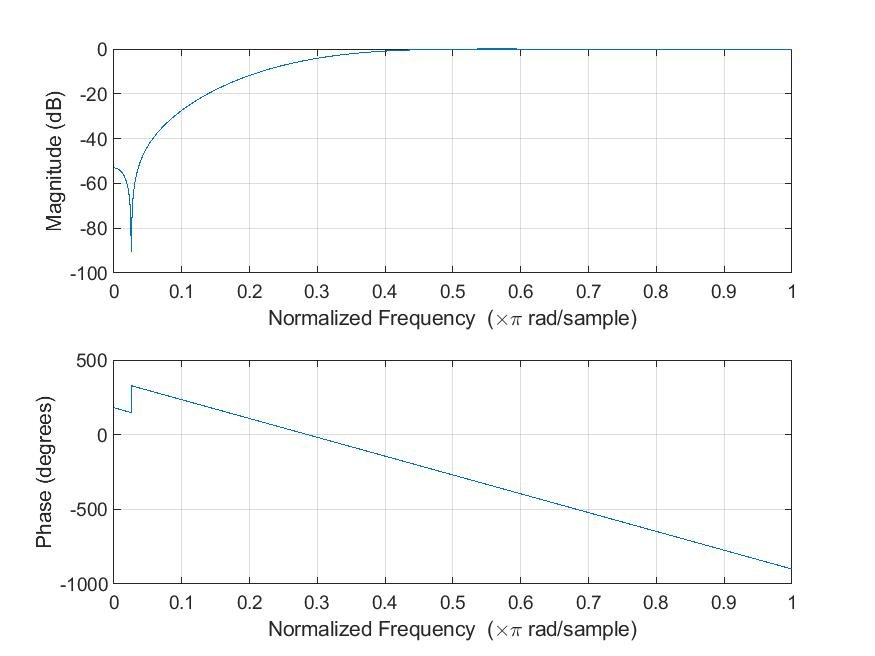
\includegraphics[scale=0.3]{stm32_fir_pasa_alto_2.jpg}

\textbf{Coeficientes preparados para el microcontrolador}\newline

	\lstinputlisting[language=c, frame=single]{../design_matlab/output/stm32_fir_pasa_alto_coef.txt}				

	
\end{document}
